\chapter{绪论}
\chaptermark{绪论}
	\section{研究背景}

	\subsection{人工智能的发展}
 	无孔不入的人工智能,别应用在各个领域,比如谷歌传统的搜索和广告业务、无人驾驶汽车,以及医疗健康部门,苹果Siri:为你解决问题的人工智能,应用了人工智能的百度外卖,代替人工顾问的智能应用,作为医疗辅助等。从互联网巨头到初创企业,都将人工智能作为发展的核心,如果关注这方面的新闻,应该看到过这样的一些新闻,"百度以近12亿元剥离游戏业务","央行成立金融科技委员会:用人工智能、云计算丰富监管手段",”苹果斥资2亿美元收购人工智能公司Lattice“等。人工智能变得越来越重要,两会期间,讯飞科大的语音识别及人工智能产品展示时,赢得了一众喝彩。 人工智能不仅涉及到民用,也涉及国家各个核心战略领域。国家主席习近平“一带一路“中演讲。他表示,“一带一路”建设要坚持创新驱动发展,加强在数字经济、人工智能、纳米技术、量子计算机等前沿领域的合作,推动大数据、云计算、智慧城市建设,连接成二十一世纪的数字丝绸之路。在这个人工智能到来的时代,发展人工智能变得越发重要。无论在国内国外,人工智能的发展都被寄予厚望。
	

		\subsection{深度学习的走红}
	随着人工智能的迅速走红,深度学习一词也迅速走红。人工智能是应用范畴的词汇,机器学习是一种实现人工智能的方法,深度学习是一种实现机器学习的方法,也是现有机器学习方法中,最奏效的一类。三者的关系见图1-1,人工智能是最外面的,下来是机器学习,最里面的是深度学习。而计算机视觉是机器学习应用最成功的一个方面,发展最为迅猛的一个分支。计算机视觉在很多方面都有应用,最为大家熟知的有人脸识别,组织恶意软件,语音识别,	无人驾驶汽车,在生物,医学方面也都有一定的应用,实际上,思科的一个评估显示,在2016年互联网上超过85\%的信息都会是像素形式,我们进入“多媒体”时代,视觉的时代,图片和视频的时代。由于互联网作为信息的载体,以及大量(视觉)传感器引发了视觉信息的大爆炸。CS231a深度学习与计算机视觉课程开篇,李菲菲教授讲计算机视觉(CV)她将这些视觉信息称为“互联网中的暗物质”,并且举了YouTube的一个例子,我们没法对这么大量的数据进行浏览,标记,分类,索引等,但是使用计算机视觉技术能够对照片进行标签、分类、处理视频中的每一帧,自动截取出篮球比赛中----比如说科比的一次精彩进球,我们现在面临着的问题就是,大量的数据,以及这些“暗物质”的挑战。目标识别与检测作为计算机视觉的一个应用,是很有应用价值的问题,而且是很多问题的根本解决之策。
	\begin{figure}[!ht]
		\centering
		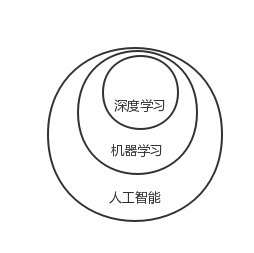
\includegraphics[width=0.3\textwidth]{figures/1-1}
		\caption{人工智能,机器学习,深度学习三者的关系图}
	\end{figure}
		\subsection{TensorFlow的出现}	
	2015年11月,谷歌宣布TensorFlow开源,由于其灵活的架构可以在一个或多个CPU,GPU、桌面、服务器、以及移动设备上部署,还不用重新编写代码,其分布式计算的方法大大缩短了机器学习的训练时间,核心代码是C++编写的简化了线上部署的复杂度,还有Python、GO、Java的接口,用户可以很容易的使用,可视化的TensorBoard,极快的编译速度,并行计算模式等优点,使其作为一个开源软件库,刚开源第一个月就积累了10000+的star,而到现在star数已经到了56939, 是GitHub上最受欢迎的深度学习框架。在图形分类、音频处理、推荐系统和自然语言处理等场景下都有丰富的应用。最近流行的Keras框架底层默认使用TensorFlow,著名的斯坦福CS231n课程使用TensorFlow作为授课和作业的编程语言,而且现在除了谷歌内部大规模使用之外,优步(Uber)、Twitter、京东、小米、FaceBook等都在使用。TensorFlow的contrib.learn模块提供了一个让开发人员从scikit-learn或Keras进入到TensorFlow的桥梁,避免了从一个框架转移到另一个框架的无措感。TensorFlow的出现使更多对机器学习感兴趣的人可以去涉足这个领域,而不是因为电脑硬件的问题,机器学习训练时间过长的问题驻足。
	人工智能,机器学习,深度学习,TensorFlow成为越来越受欢迎的话题,我在百度指数,以及Google trends上,分别输入了机器学习,深度学习,还有人工智能几个搜索词后,得到的搜索热度趋势图见图1-2。通过这些数据得出的结论是人工智能,深度学习,正在变得越来重要,正在引起越来越多的重视。而在Google trends中看到TensorFlow搜索热度趋势图见图1-3 。TensorFlow的热度基本维持在100,足以说明这是目前很受欢迎的一个话题。
	\begin{figure}[!ht]
		\centering
		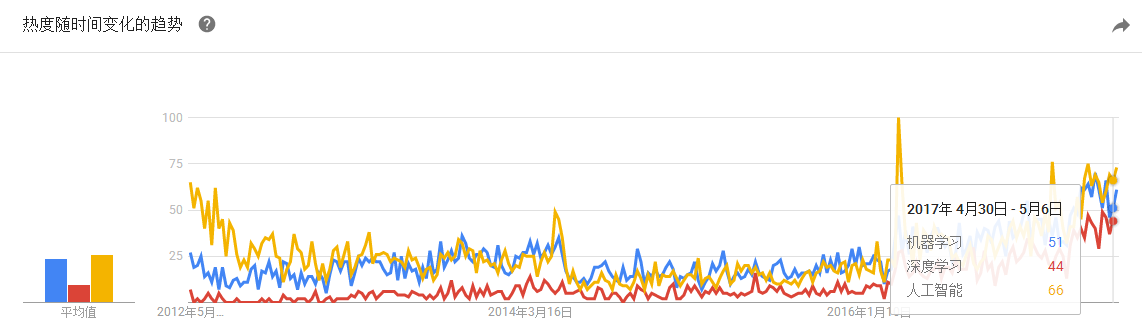
\includegraphics[width=0.5\textwidth]{figures/1-2}
		\caption{Google trends搜索热度趋势图}
	\end{figure}
	\begin{figure}[!ht]
	\centering
	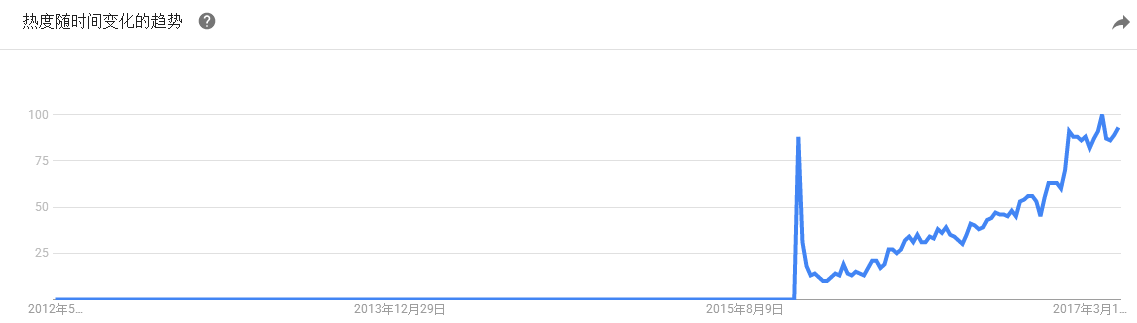
\includegraphics[width=0.5\textwidth]{figures/1-3}
	\caption{TensorFlow 在谷歌搜索的热度趋势}
	\end{figure}
	\section{研究意义和目标}
		\subsection{研究意义}
		在人工智能大火的时代,作为其细小分支的计算机视觉发展趋势也在变得良好。计算机视觉最初开始于29世纪70年代,当时计算机视觉被视为人工智能的感知部分,到2012年,深度学习的出现,在此之前的是十年期间计算机视觉领域就如何用特征来建模进行研究,传统的机器学习算法(SVM等),深度学习的出现使计算机视觉的研究有了新的进展。参考图1-4图1-5可以大致了解一下计算机视觉1966年开始的发展史。作为人工智能中发展速度最快的一个分支,与计算机视觉相关的领域交叉学科较为活跃,智能手机,电商,无人驾驶汽车,无人机等,在军事,医学方面也都有应用。深度学习,大量的数据,硬件(CPU、GPU)的支持,计算机视觉被应用在很多产品和应用场景之中。计算机视觉的增强,可以改善我们的生活,可以让机器代替人类去完成更多的任务,比如,24小时的场景监控,Placemete传感器(已经可以识别5种物体了)。
		\begin{figure}[!ht]
			\centering
			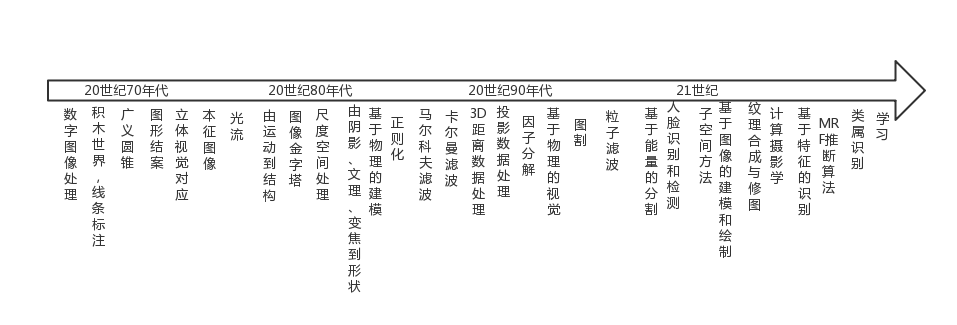
\includegraphics[width=0.5\textwidth]{figures/1-4}
			\caption{计算机视觉发展史时间图}
		\end{figure}
		\begin{figure}[!ht]
			\centering
			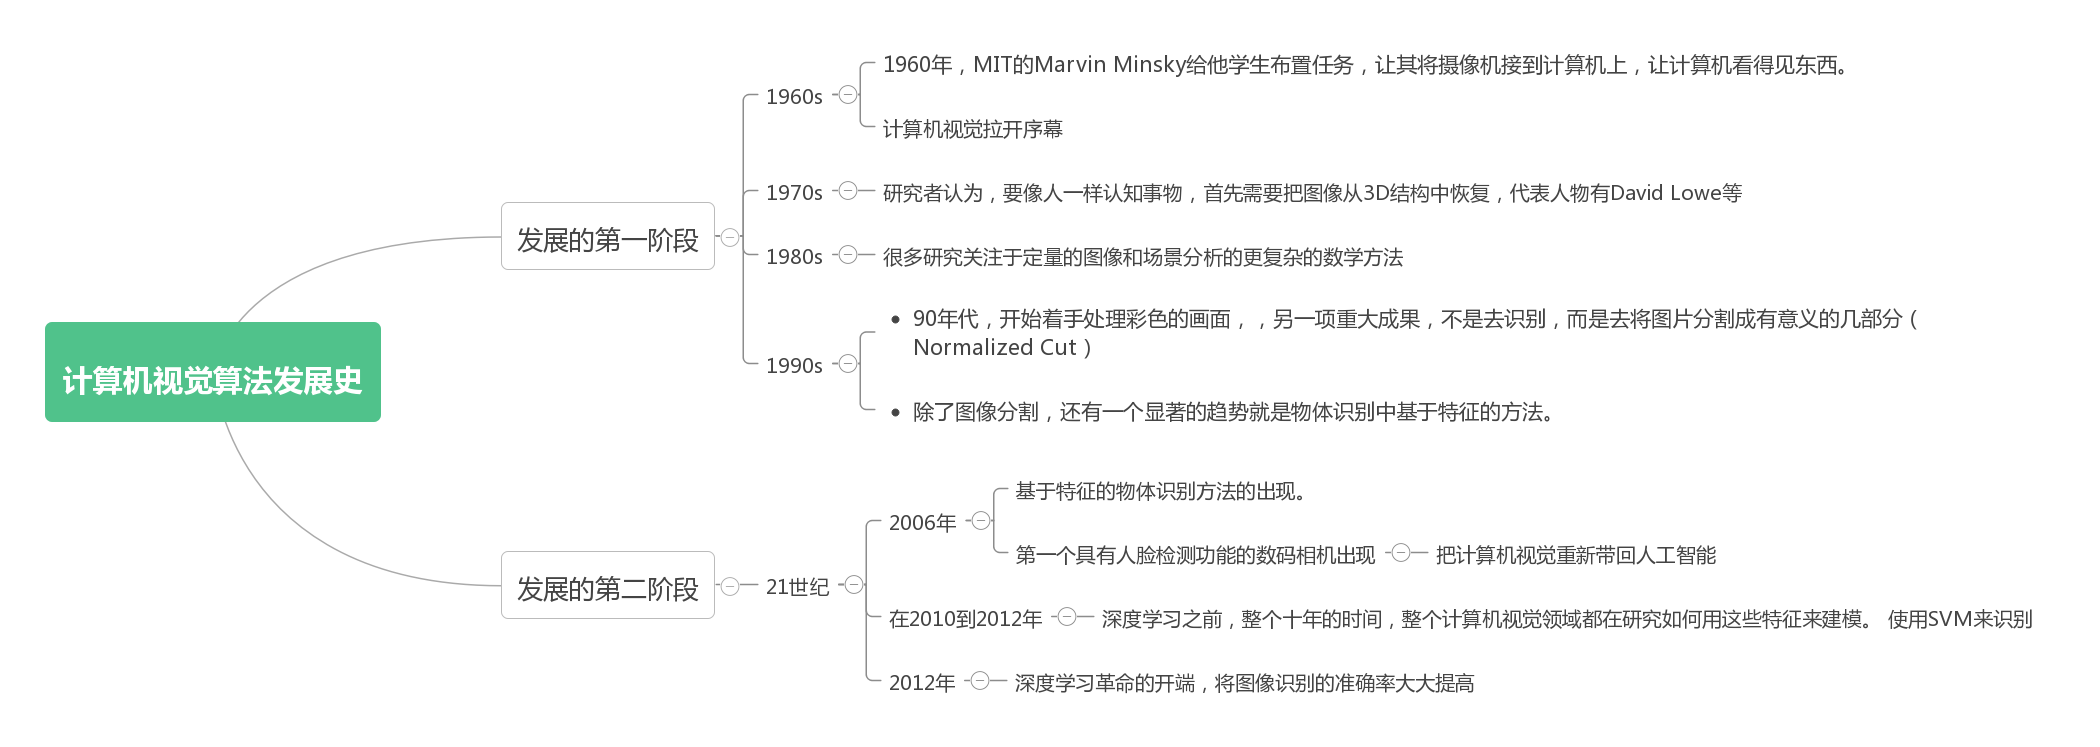
\includegraphics[width=0.5\textwidth]{figures/1-5}
			\caption{计算机视觉发展史思想变化图}
		\end{figure}
		
		在目标的检测中有三个很重要的要素(1)识别准确度(2)识别效率(3)定位准确。大量的数据可供训练,以及深度学习的出现发展,可以大大提升识别精准度,数据量对精准度的影响见图三,深度学习发展对精准度的影响见图4,现在的数据量已经要达到亿GB级别,并且还将持增长趋势。GPU对数据的处理能力远高于传统的CPU,对于对数据处理有极高要求的计算机视觉来说由于数据处理已经不能成为一个问题,而且TensorFlow由于其各种优点(后面会有介绍)也改善了这个问题,大大缩短了训练时间,还可以在CPU上进行训练;国家政策的支持,企业的发展需求,以及企业投资热度来看,还是由于目标的识别与检测是CV众多任务中最有挑战性,且应用很广,目标识别与检测都是一个值得研究的话题。
		
	
		而对于我们来说作为一个农科大,就不得不关注一下在农业方面的应用了,就查到了专注于研究无人机的北醒光子科技公司,最近的雷达产品是被用于植保无人机的,与传统植保无人机不一样的是,该无人机能够通过识别农作物顶端细微的高度差别来进行飞行高度调整,来确保对于不同高度作物的农药喷洒效果可以达到基本一致。以及耿琪超(85后创客)用了三年时间研发出来的可用于智能化分拣蔬菜的机器人等。
		\begin{figure}[!ht]
			\centering
			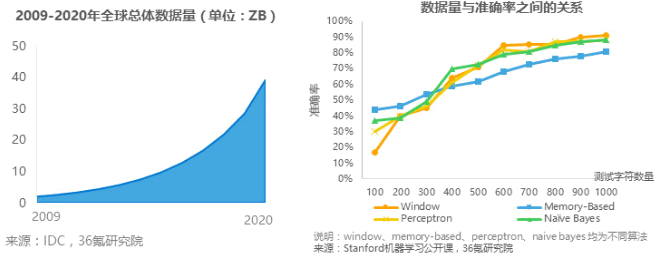
\includegraphics[width=0.5\textwidth]{figures/1-6}
			\caption{深度学习影响比率}
		\end{figure}
		\begin{figure}[!ht]
			\centering
			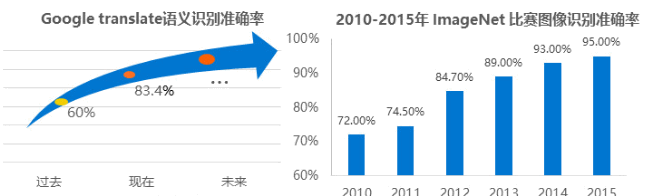
\includegraphics[width=0.5\textwidth]{figures/1-7}
			\caption{深度学习图像准确率}
		\end{figure}
	
	计算机视觉作为人工智能的基础应用,投资热度只增不减,而且就像上文提到的它的应用场景很广,从人工智能兴起迎来创业高峰的时候,计算机视觉作为其中创业热度很高领域,2014到2015年期间初创公司的数量增加,与人工智能领域整体趋势差不了太多。且公司的平均年龄大概为3.9左右。
	应用场景简介:
	通用的计算机视觉主要指的是底层技术开发,主要用来解决各种的场景识别问题,包括图像识别平台以及嵌入式的视觉软件,具体地包括以下几个方面人像识别、物体识别、手写字符识别、表情识别、视频对象提取以及场景识别等。应用到具体的产品中就包括监视、视频分析、机器人、搜索引擎等。技术成熟度CV各细分领域不太一样,在生物特征的识别方面较为成熟,比如人脸识别,指纹识别等,但是物体和场景的识别中成熟度就较为低,仍然在探索中,但是对静态图片与动态图片的成熟度又是不一样的。大概是受到图片质量以及光照的因素的影响吧。
	市场规模:
	CV的应用场景广,必然引起的结果就是市场潜力很大,而CV公司数量又是相当多的,人脸识别和监控作为作为其中很重要的应用,其市场规模也是相当大的参考Capvision,以及36氪研究院的数据,如图1-8显示表明中国视频监控的市场规模变化趋势图(亿为单位)。可以看出市场容量是相当大的。
	\begin{figure}[!ht]
		\centering
		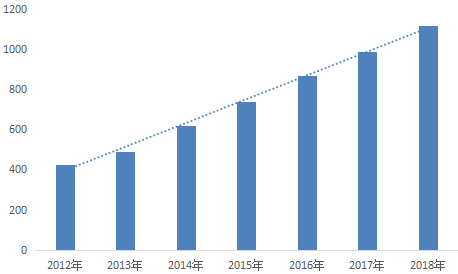
\includegraphics[width=0.5\textwidth]{figures/1-8}
		\caption{市场规模变化趋势}
	\end{figure}
		\subsection{研究目标}
		
	\section{本文研究内容}
		
		
	\section{本文内容安排}
	